\chapter{Giới thiệu}
\thispagestyle{fancy}
\section{Đặt vấn đề}
Theo ước tính của Tổ chức Y tế thế giới, hàng năm trên thế giới có khoảng 17,5 triệu người tử vong do các bệnh liên quan đến tim mạch và số bệnh nhân tim mạch tích lũy ngày một nhiều. Theo dự báo của Hội Tim mạch Việt Nam, khoảng 20\% dân số nước ta mắc bệnh về tim mạch và tăng huyết áp. Tỷ lệ tăng huyết áp ở những người trẻ từ 25 tuổi đang gia tăng, chiếm 21,5\% tổng số ca mắc bệnh.

% \begin{center}
%     \begin{figure}[htp]
%     \begin{center}
%     
\includegraphics[scale=.4]{image/chapter0/benh-tim-mach-2_0003323_710.jpeg}
%     \end{center}
%     \caption{Số người mắc bệnh tim mạch ngày càng tăng}
%     \end{figure}
% \end{center}
Tuy nhiên, vẫn còn nhiều người thờ ơ, chủ quan và thiếu quan tâm đến sức khoẻ tim mạch của mình. Theo thống kê của Hội tim mạch Việt Nam, vào năm 1980, tỷ lệ mắc bệnh tim mạch ở tuổi 50 trở lên chỉ ở mức 11\%, thì đến năm 2009, tỷ lệ này lên đến 25\% và độ tuổi mắc từ 22 tuổi trở lên\cite{baibao}. Bất thường ở tim mạch có nhiều loại, trong số đó đặc biệt phải nói đến chứng Rối loạn nhịp tim. Rối loạn nhịp tim là một bệnh tim đặc trưng bởi tần số hoặc nhịp tim bất thường: quá nhanh, quá chậm, quá sớm hoặc quá thất thường. Đồng thời bệnh thường phổ biến hơn nhiều với nam giới (70\% các trường hợp), và 30\% bệnh nhân là nữ (theo nghiên cứu thuộc Khoa Y, Trường Cao đẳng Y tế Baroda, Bệnh viện Đa khoa Sir Sayaji, Vadodara, Ấn Độ) \cite{rlnt}.

Rối loạn nhịp tim có thể không có triệu chứng hoặc chỉ gây ra các triệu chứng như: đánh trống ngực, cảm giác đột ngột xuất hiện cơn khó thở - cảm giác khó chịu ở ngực đi kèm,chóng mặt,... Tuy nhiên nhiều trường hợp rối loạn nhịp có thể đe doạ tính mạng của người bệnh và khiến người bệnh phải nhập viện trong tình trạng cấp cứu.

Bệnh có thể gặp ở mọi lứa tuổi và gặp ở cả hai giới, tuy nhiên theo các nghiên cứu thống kê thì bệnh lý rối loạn nhịp gặp nhiều hơn ở các đối tượng sau: tuổi trên 60, người bệnh tăng huyết áp, bệnh động mạch vành, suy tim, bệnh lý van tim, tiền sử phẫu thuật tim mở, ngừng thở khi ngủ, bệnh lý tuyến giáp, đái tháo đường, bệnh phổi mạn tính, lạm dụng rượu hoặc sử dụng chất kích thích, tình trạng nhiễm trùng hoặc bệnh lý nội ngoại khoa nặng...

Việc kiểm tra tim mạch định kì là rất cần thiết theo nhiều khuyến cáo của bộ y tế, tuy nhiên để đo điện tim thì một người phải vào các cơ sở y tế với các thiết bị chuyện dụng, phải thực hiện nhiều kiểm tra, xét nghiệm, cách làm này tốn khá nhiều thời gian và tiền bạc dẫn đến hậu quả là số ca mắc các bệnh tim mạch ngày càng gia tăng và có những biến chứng nguy hiểm.

\section{Mục tiêu}
% \begin{center}
%     \begin{figure}[htp]
%     \begin{center}
%     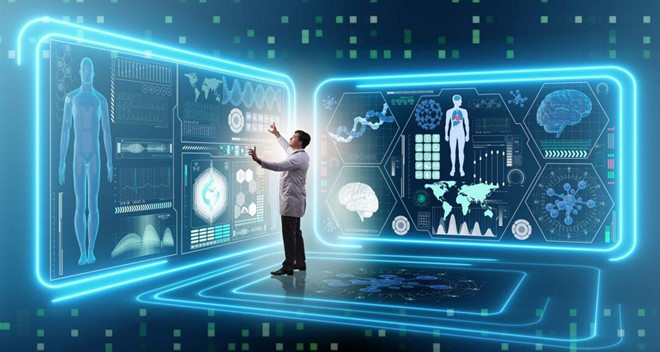
\includegraphics[scale=.4]{image/chapter0/r_sfcc.jpg}
%     \end{center}
%     \caption{Trí tuệ nhân tạo đang phát triển vượt bậc và có nhiều thành tựu trong y khoa}
%     \end{figure}
% \end{center}
Trí tuệ nhân tạo là sự "tư duy" của máy móc, trong đó các thiết bị sẽ bắt chước cách tư duy tự nhiên của con người để giải quyết các vấn đề. Trong cuộc cách mạng công nghiệp 4.0, AI là một trong những yếu tố then chốt. Từ khái niệm tưởng chừng xa xôi, trí tuệ nhân tạo từng bước đi vào đời sống, hiện thực hóa giấc mơ về những loại máy móc có khả năng tư duy như con người. Bên cạnh đó những năm trở lại đây công nghệ internet vạn vật cũng rất phát triển, một vấn đề ta thường nghe nói đến tình trạng quá tải tại các bệnh viện, bệnh nhân không có đủ giường bệnh đề nằm. Sắp tới đây sự ra đời của những chiếc giường thông minh sẽ tạo cảm giác thoải mái tối ưu cho bệnh nhân. Những chiếc giường có thể phát hiện các chuyển động của bệnh nhân và điều chỉnh chiều cao cho phù hợp mà không cần y tá hay can thiệp của con người. Ngoài ra trong thời gian sắp tới sẽ có rất nhiều những thiết bị thông minh ra đời hỗ trợ cho hoạt động khám chữa và điều trị bệnh tại các bệnh viện, phòng khám. Với công nghệ IoT bắt đầu được triển khai ở khắp mọi nơi, sẽ mang lại kết quả tuyệt vời bằng cách giảm chi phí, cải thiện kết quả điều trị, tăng cường trải nghiệm bệnh nhân, giảm lỗi, tăng cường quản lý thuốc và cải thiện quản lý bệnh tật.

Hứa hẹn về ứng dụng của công nghệ trí thông minh nhân tạo (AI) trong ngành y tế là rất lớn, nhiều ứng dụng của trí tuệ nhân tạo vào trong ngành y tế đem lại những thành tựu đáng kể như: robot phẫu thuật có trí thông minh nhân tạo, trợ lý y tá ảo, hỗ trợ đưa ra phác đồ điều trị ung thư,... Vì thế việc áp dụng trí tuệ nhân tạo vào lĩnh vực tim mạch, phát hiện sớm những dấu hiệu bất thường của tim đóng vai trò rất quan trọng giúp giảm nguy cơ mắc các bệnh tim mạch. Trong đó một trong những phương pháp để phát hiện bệnh là đo điện tim. Điện tim là một trong những phương pháp thể hiện rõ nhất những dấu hiệu của tim, điện tim giúp cho bác sĩ phát hiện các bệnh lý như đau ngực, rối loạn nhịp tim, nhồi máu cơ tim, hở van tim, thiếu máu cơ tim,... thông qua việc ghi lại những tín hiệu xung điện qua tim theo một đường truyền dẫn, chúng được hình thành từ các tế bào trong hệ thống cơ tim khi tim hoạt động. Thu thập tín hiệu điện tim từ các thiết bị IoT tiếp qua một hệ thống phân loại để phát hiện sớm các bất thường ở điện tim một cách nhanh chóng và tương đối chính xác sẽ góp phần giám thiểu nguy cơ mắc bệnh tim mạch. Mục tiêu của để tài là sử dụng một hệ thống phân loại sử dụng các kỹ thuật học sâu (Deep Learning) để phát hiện loại bất thường ở điện tim.

